%\documentclass[draft]{beamer}%\documentclass[]{beamer}
\documentclass[]{beamer}%\documentclass[draft]{beamer}
\mode<presentation>
{
%  \usetheme{Boadilla}
  \usetheme{Frankfurt}
  \usecolortheme{crane}
}
\usepackage{graphicx}
%~ \usepackage{cite}
\usepackage{hyperref}


\setbeamerfont{fig_font}{size=\small}
\setbeamercovered{invisible}
\usefonttheme[onlysmall]{structurebold}
% Delete this, if you do not want the table of contents to pop up at
% the beginning of each subsection:
% \AtBeginSubsection[]
% {
%   \begin{frame}<beamer>{Outline}
%     \tableofcontents[currentsection,currentsubsection]
%   \end{frame}
% }

% End Beamer stuff
\begin{document}
\title{Project Presentation: A ID 408 Report by Group 07.}
\setbeamerfont{author}{size=\scriptsize,series=\bfseries,parent=structure}
\author{Utkarsh Kumar, 130050022 \linebreak \\
		utkarshk@cse.iitb.ac.in \linebreak \\
		Ankit Rathod, 130050029 \linebreak \\
		rathod.ankit@cse.iitb.ac.in \linebreak \\
		Ashish Anand, 130050035 \linebreak \\
		ashishanand@cse.iitb.ac.in \linebreak \\
		Dibyendu Mondal, 130050046 \linebreak \\
		dibyendu@cse.iitb.ac.in \linebreak \\
}
\date{November 17, 2014}

\begin{frame}
\titlepage
\end{frame}



\section{Overview}

\begin{frame}
\frametitle{Overview}
\begin{columns}
\begin{column}{.5\textwidth}
\begin{itemize}
\item Introduction
\item What Happens
\item Description of components
\item Conclusion
\item Bibliography
\end{itemize}
\end{column}
\begin{column}{.5\textwidth}

\includegraphics[width=.7\textwidth]{Box2d}
\end{column}
\end{columns}
\end{frame}


\section{Introduction}

\begin{frame}
\frametitle{Introduction}
This report has been made to present the working of the Rube-Goldberg machine simulation made by our group (group no 07) using Box2D. \
We have included screenshots to explain different parts of the entire picture. Also explanations for what happens in which particular part have been given.
\end{frame}

\section{What Happens}

\begin{frame}
\frametitle{What Happens}
\begin{columns}
\begin{column}{.7\textwidth}
\begin{scriptsize}
The man on the right holds the man on the left at gun point. The man being held at gun point kicks a small ball which sets off a chain of events. \
The simulation starts at the point when the man just kicks the ball. In this picture, the ball kicked moves down, to hit the balanced bar which stops 2 balloons. \
This disturbs the balance and one of the balloons goes up to hit the platform above, which slightly tilts it to make the three balls placed on it to roll over to \
the right side.
\end{scriptsize}
\end{column}
\pause
\begin{column}{.4\textwidth}
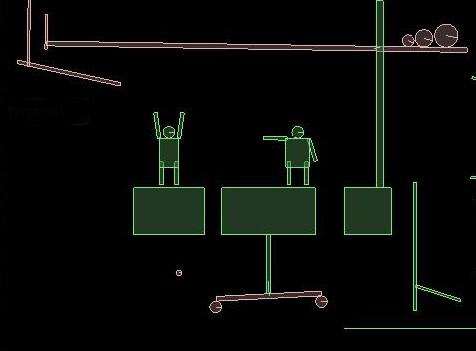
\includegraphics[width=4.5cm,height=3cm]{wh1}
\end{column}
\end{columns}
\end{frame}

\begin{frame}
\frametitle{What Happens}
\begin{columns}
\begin{column}{.7\textwidth}
\begin{scriptsize}
Then, these balls go and fall into holes of appropriate sizes making a way for the next balls to pass over them. The smallest of these balls continues down the path \
and finally hits the series of dominoes which fall over and nudge a vertical rotating bar which further makes the series of dominoes on the upper level fall over each other.\
\end{scriptsize}
\end{column}
\pause
\begin{column}{.4\textwidth}
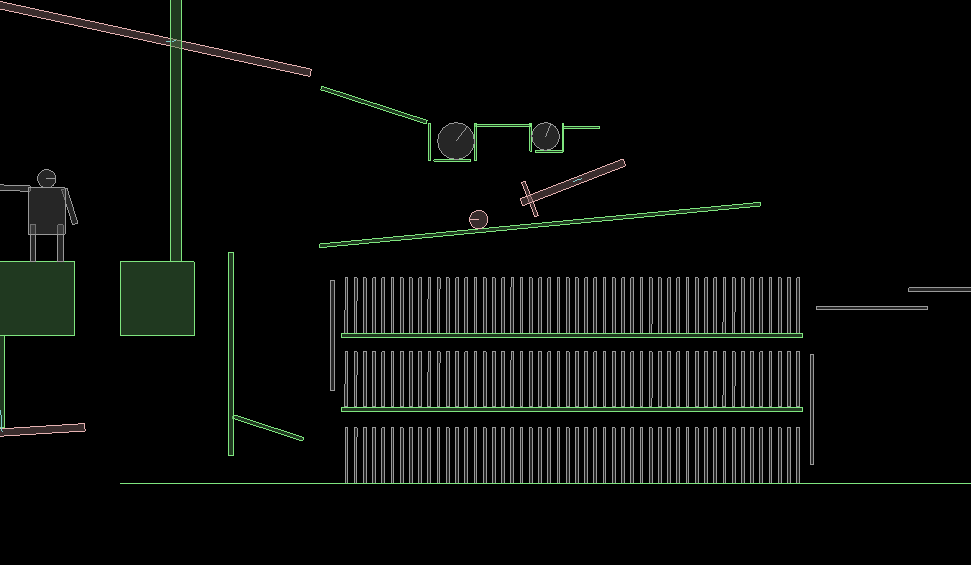
\includegraphics[width=4.5cm,height=3cm]{wh15}
\end{column}
\end{columns}
\end{frame}

\begin{frame}
\frametitle{What Happens}
\begin{columns}
\begin{column}{.7\textwidth}
\begin{scriptsize}
Then, these balls go and fall into holes of appropriate sizes making a way for the next balls to pass over them. The smallest of these balls continues down the path \
and finally hits the series of dominoes which fall over and nudge a vertical rotating bar which further makes the series of dominoes on the upper level fall over each other.\
\end{scriptsize}
\end{column}
\begin{column}{.4\textwidth}
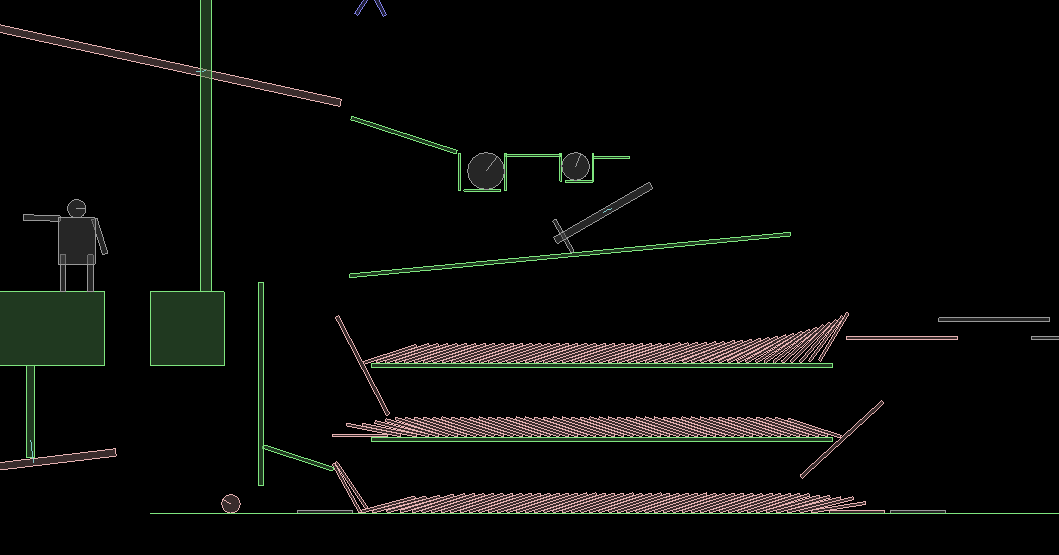
\includegraphics[width=4.5cm,height=3cm]{wh2}
\end{column}
\end{columns}
\end{frame}


\begin{frame}
\frametitle{What Happens}
\begin{columns}
\begin{column}{.7\textwidth}
\begin{scriptsize}
The last domino on the top level topples over the horizontal roating bar next to it and the motion gets transferred through a series of bars finally ending up tilting the \
bar on which the large ball is kept. This ball falls into the platform below which is connected to a block on the other side of the pulley, making it rise up.
\end{scriptsize}
\end{column}
\pause
\begin{column}{.4\textwidth}
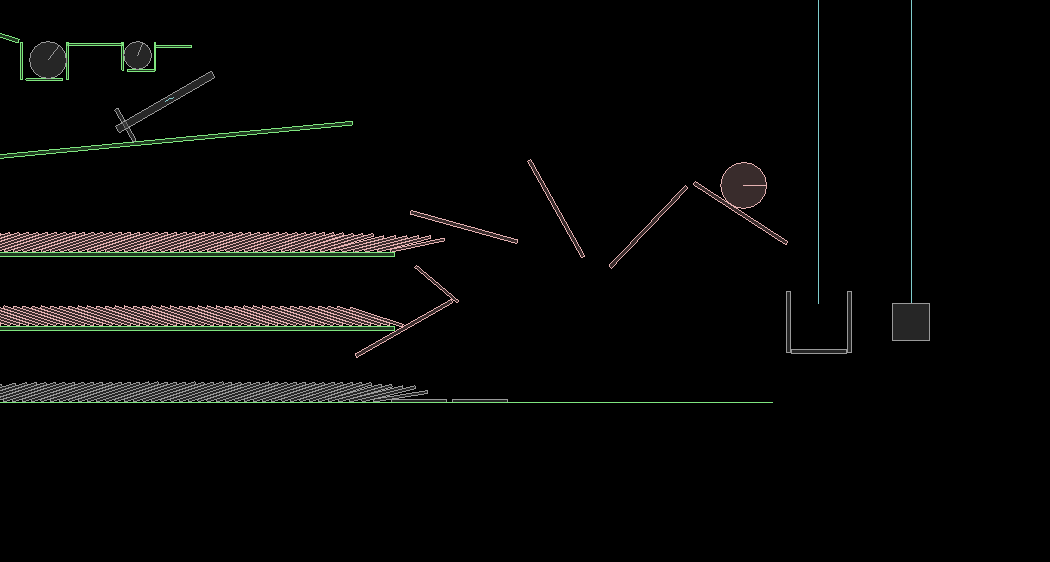
\includegraphics[width=4.5cm,height=3cm]{wh3}
\end{column}
\end{columns}
\end{frame}

\begin{frame}
\frametitle{What Happens}
\begin{columns}
\begin{column}{.7\textwidth}
\begin{scriptsize}
The block hits the series of rotating four handled objects and the motion gets transmitted to the right most ball on the top platform. This ball then moves left, hitting \
the next ball and this continues till the last ball.
\end{scriptsize}
\end{column}
\pause
\begin{column}{.4\textwidth}
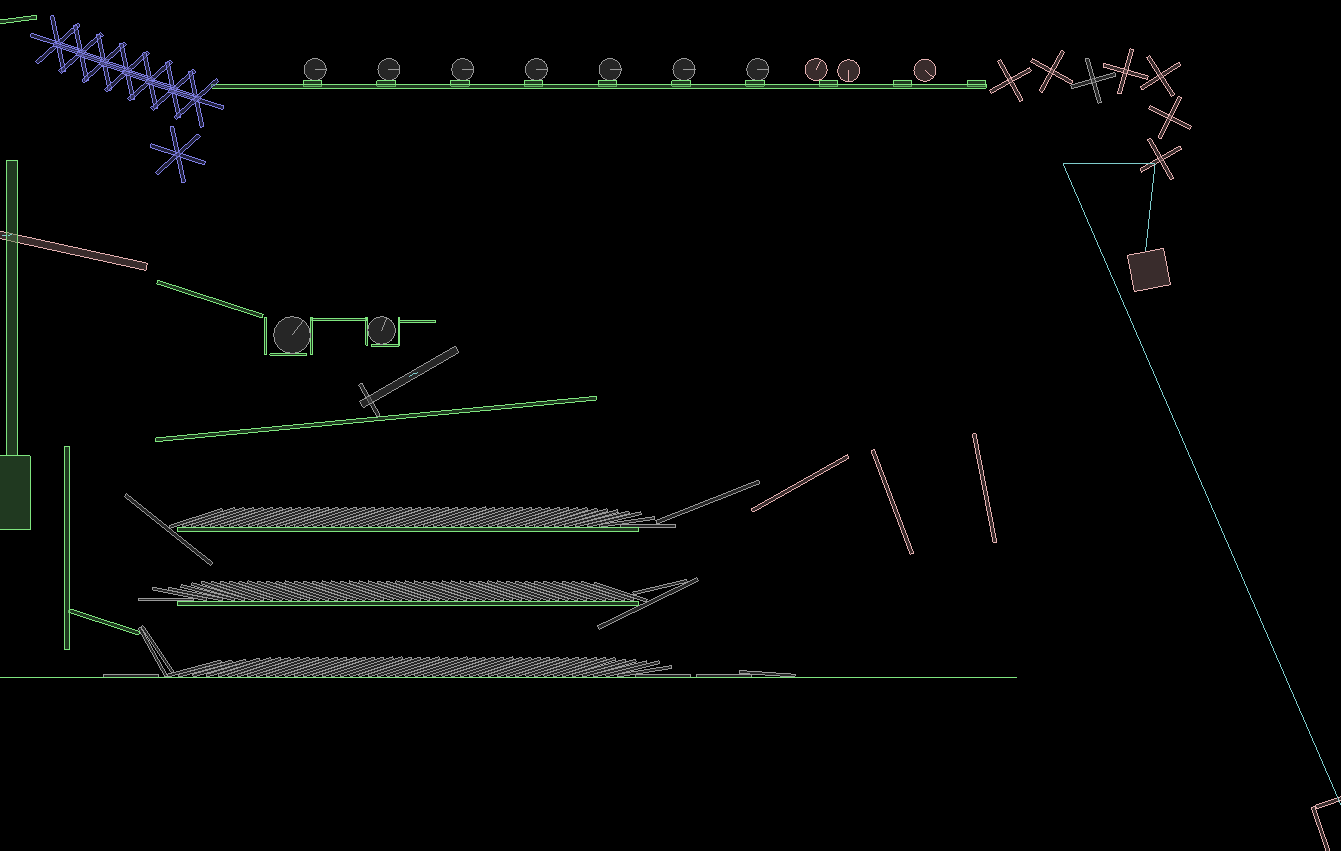
\includegraphics[width=4.5cm,height=3cm]{wh45}
\end{column}
\end{columns}
\end{frame}

\begin{frame}
\frametitle{What Happens}
\begin{columns}
\begin{column}{.7\textwidth}
\begin{scriptsize}
The last ball, when it reaches the end of the platform, lands on an array of rotators which push it up to the next platform. It then, rolls down the incline into the tunnel \
that follows. 
\end{scriptsize}
\end{column}
\pause
\begin{column}{.4\textwidth}
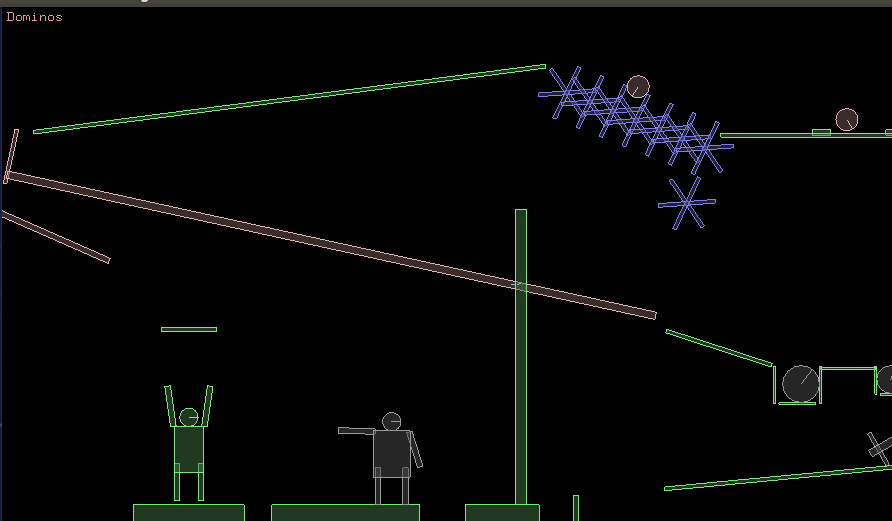
\includegraphics[width=4.5cm,height=3cm]{wh5}
\end{column}
\end{columns}
\end{frame}

\begin{frame}
\frametitle{What Happens}
\begin{columns}
\begin{column}{.7\textwidth}
\begin{scriptsize}
The ball comes out at the other end of the tunnel and falls on the man with the gun, thus, knocking him over.
\end{scriptsize}
\end{column}
\pause
\begin{column}{.4\textwidth}
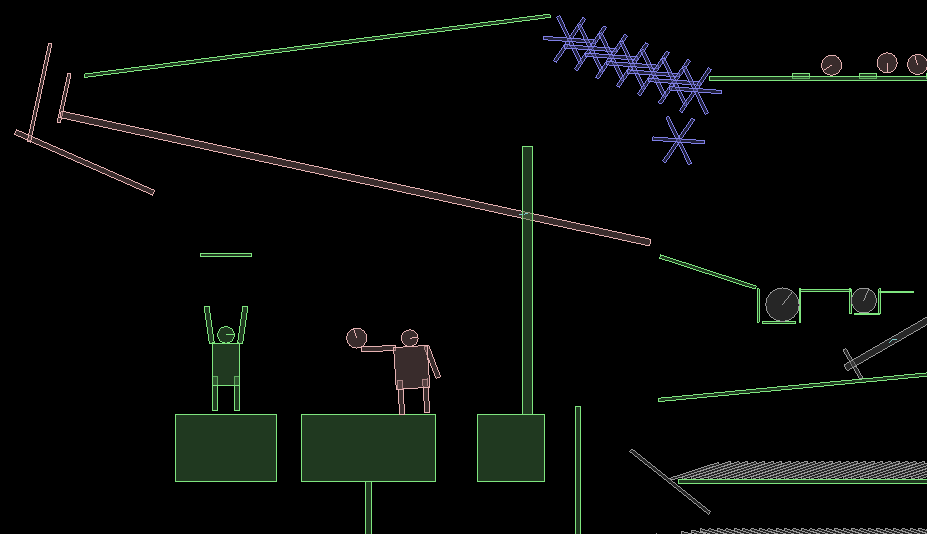
\includegraphics[width=4.5cm,height=3cm]{wh6}
\end{column}
\end{columns}
\end{frame}



\section{Body}

\begin{frame}
\frametitle{Description of components}
The following are the major components of our project version 1.0:
\begin{itemize}
\item Dominoes \pause
\item Pulley system \pause
\item Array of rotators
\end{itemize}
\end{frame}

\subsection{Dominoes}
\begin{frame}
\frametitle{Description of components}
\framesubtitle{Dominoes}
\begin{columns}
\begin{column}{.7\textwidth}
\begin{scriptsize}
The dominoes have been made using an array of of rectangular blocks placed close to each other such that when one falls, it makes the next fall and so on.
\linebreak
\pause
The dominoes are dynamic bodies, whose initial position has been defined to be on top of the stationary shelves(which are static objects. For more information \
about different types of objects in box2d, see ~\cite{Site1} or ~\cite{Site2}.
\end{scriptsize}  
\end{column}
\begin{column}{.4\textwidth}
\pause
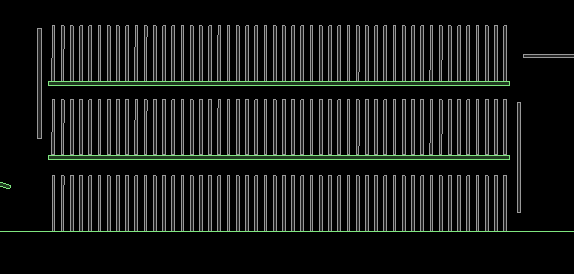
\includegraphics[width=4.5cm,height=3.3cm]{dd1}
\end{column}
\end{columns}


\end{frame}




\subsection{Pulley system}

\begin{frame}

\frametitle{Description of components}
\framesubtitle{Pulley System}
\begin{columns}
\begin{column}{.7\textwidth}
\begin{scriptsize}
The pulley system has an open box at one end and a square block at the other. The open box catches a ball when it falls into it.
\pause
\linebreak
The open box and the block are dynamic bodies and they have been connected via a pulley joint. More about different types of joints can be found at ~\cite{Site1} or ~\cite{Site2}.
\end{scriptsize}  
\end{column}
\begin{column}{.4\textwidth}
\pause
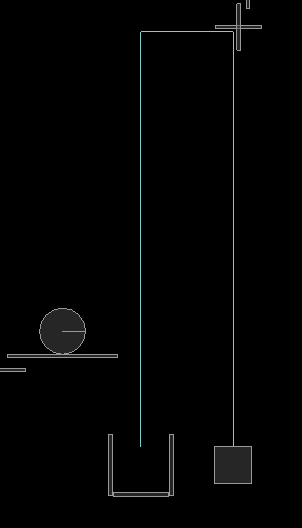
\includegraphics[width=3cm,height=5cm]{dd2}
\end{column}
\end{columns}

\end{frame}


\subsection{Array of Rotators}

\begin{frame}

\frametitle{Description of components}
\framesubtitle{Array of Rotators}
\begin{columns}
\begin{column}{.7\textwidth}
\begin{scriptsize}
The array of rotators is an array of kinematic bodies which have been given a constant angular velocity and their hinge point has been defined by fixture-less bodies. More \
about kinematic bodies can be found at ~\cite{Site3} 
\end{scriptsize}  
\end{column}
\begin{column}{.4\textwidth}
\pause
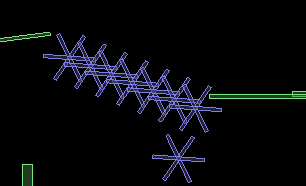
\includegraphics[width=4.5cm,height=2.8cm]{dd3}
\end{column}
\end{columns}

\end{frame}


\section{Conclusion}

\begin{frame}
\frametitle{Conclusion}
In this presentation, we saw how Box2D can be used to model physical systems on a computer, of which an example is our Rube-Goldberg machine simulation version 1.0.\ 
Different aspects of the Box2D physics engine were demonstrated and a realistic simulation was carried out.
\end{frame}



\section{References}


%\begin{frame}
%\frametitle{References}
%\begin{itemize}
%\item Stoke's law and viscosity: \url{http://www.britannica.com/EBchecked/topic/567002/Stokess-law}
%\item Conservation of angular momentum: \url{http://www.sparknotes.com/physics/rotationalmotion/angularmomentum/section2.rhtml}
%\item Solution of a simple pulley system: \url{http://courses.ncssm.edu/apb10/resources/guides/G06-1.net_force_system.htm}
%\end{itemize}
%\end{frame}

\begin{frame}
\frametitle{References}
\bibliography{main}{}
\bibliographystyle{alpha}
\end{frame}


\end{document}

%\input{reference.tex}
%~ \bibliographystyle{
\end{document}

